\chapter{Event Selection \& Background Estimation} \label{chap-EventSelection}

\section{Event Selection}

Skim

\section{Trigger and Event Cleaning}

\subsection{Trigger selection}

As the $t\bar{t}+\gamma$ analysis is studied as a di-lepton final state, the requirement of at least two oppositely charged leptons (electrons or muons only) is essential. These datasets are identified by the trigger system (as described in Section \ref{sec-Trigger}) to contain two leptons. Triggers are generally divided into two categories; single object triggers fire on one or more objects of the same flavour passing certain preselection requirements, such as p$_T$ and $\eta$, and cross-triggers which select two objects of different flavours as predetermined by the user. For this analysis, both types of triggers are implemented in order to select the three final states in question. The list of trigger paths can be seen in Table \ref{tab-HLTriggers}. 

\begin{table} \label{tab-HLTriggers}
\begin{center}
\begin{tabular}{|c|p{11.5cm}|}
\hline
	\textbf{Final State} & \textbf{High Level Trigger Path} \\
\hline
	$\mu^+\mu^-$ & HLT\_Mu17\_Mu8\_v* \\
	$e^+e^-$ & HLT\_Ele17\_CaloIdT\_CaloIsoVL\_TrkIdVL\_TrkIsoVL
				\_Ele8\_CaloIdT\_CaloIsoVL\_TrkIdVL\_TrkIsoVL\_v* \\
	$e\mu$ & HLT\_Mu17\_Ele8\_CaloIdT\_CaloIsoVL\_TrkIdVL\_TrkIsoVL\_v*, HLT\_Mu8\_Ele17\_CaloIdT\_CaloIsoVL\_TrkIdVL\_TrkIsoVL\_v*s \\
\hline	
\end{tabular}
\caption{Triggers for each di-lepton channel.}
\end{center}
\end{table}

Each trigger path name explains the selection requirements on the objects that it triggers on. The term Mu refers to a reconstructed muon and Ele refers to a reconstructed electron, where the succeeding number represents an associated energy threshold of the particle. For example, the the di-muon channel uses a single flavour object trigger to select two muons and is used with the requirements that one of the muons has a p$_T$ greater than 8 $\GeV$ and the second greater than 17 $\GeV$. The version of the trigger is denoted in the trigger path as v*, as the trigger path changes with the trigger table used. It should be noted that a different trigger version does not in fact require a change in trigger path. At this level the number of energy deposits within the calorimetry is still too large for the trigger rate to be usable, and thus extra selection requirements on the trigger system must be imposed.

A way to reduce the trigger rate is to impose cuts on the energy threshold of the particles in question greater than that required by the trigger, however this holds drawbacks for analyses who then wish to implement tighter cuts within offline analysis. Another method, and one that is used primarily in electron trigger studies, is to reduce trigger rates to a more feasible level is to introduce isolation and Id cuts, the `Iso' and `Id' terms that can be seen in the di-electron and $e\mu$ trigger path names. The objects must then also pass simple isolation and id criteria and thus reducing the trigger rate. The information for each is obtained from both the calorimeter (e.g CaloIso) and tracker (e.g TrkId) by placing requirements on such parameters as the shape of the energy cluster, the total number of energy depositions, and the angular separation between the ECAL and tracker energy deposits. Three categories of selection are implemented for each kinematic cut, and are listed as Tight (T), Loose (L), and Very Loose (VL) as can be seen in the trigger paths. These signify the harshness of the cuts when applied. This can be visualised, for example, in the the di-electron channel where the HLT calls for two electrons, where one must pass an energy threshold of 8 $\GeV$ with a tight requirement on calorimeter Id, and very loose requirements on calorimeter isolation and tracker Id and isolation. The other electron must pass an energy threshold of 17 $\GeV$ with the same calorimeter and tracker isolation and Id cuts.

HLTs are used for the $t\bar{t}+\gamma$ analysis such that if the event does not pass the requirement of the trigger, then it is not included in the calculation. Single object triggers are used for both the di-muon and di-electron channels, and two cross-triggers were used for the $e\mu$ channel as the final state selection requires two oppositely charged leptons (electrons or muons) where one is an electron and the other a muon. The triggers were processed specifically for the $\sqrt{s}=8 \TeV$ data-taking period with 19.6 $\fbinv$.

\subsection{Filtering}

Known anomalies derived from detector and accelerator effects are a prominent feature in the processing of data. To counter these effects we incorporate several `cleaning' filters after trigger selection, but before any further selection cuts are applied. The first of which vetoes on \textbf{beam scraping} and includes a \textbf{tight CSC Beam Halo Filter}. We find that, even with the accuracy and precision that the LHC provides on accelerating bunches of protons, protons have a tendency to diverge radially from the bunch and form what is known as the beam halo that circulates the accelerator with the bunch. In early analyses it was found that the beam halo particles can be picked up in the detectors and be reconstructed as being part of an event in which it is not. Due to sensitivity to beam halo particles in the muon detectors, a filter is introduced based on muon tracking kinematics and thus veto on such events. Beam halo particles can also be removed from the beam within the LHC by introducing collimating blocks around the beam line at various points on the accelerator. This, however, presents another problem in the form of showering as the particles interact with the collimator blocks, beam scraping, and be detected by the experiments. These events are accounted for and removed from analyses by introducing the requirement that at least 25\% of reconstructed tracks within the inner detector pass the high purity threshold (see Section \ref{subsec-ChargedParticleTracking}). 

Similarly, we employ a \textbf{HCAL noise filter} in order remove events with anomalous noise within the HCAL. CMS expects a certain degree of noise, stemming from the electronic of the detector, to be present when recording data, however the majority of anomalous noise is found to originate in the Hybrid Photo-Triodes (HPT) and their corresponding read-out boxes. At the current energy scale this is not a problem as the noise appears as large, isolated energy deposits. Anomalous events have easily-identifiable signatures such as the isolation and isolation of the HCAL readout, and the multiplicity in the read-out boxes. So, if a signal demonstrates very little change in the pulse shape over time, and the read-out boxes display a high multiplicity, then an event is rejected.

\textbf{HCAL laser filter}

\section{Di-lepton Selection and vetoes}

\subsection{Electrons}

\subsection{Muons}

\subsection{Photons}

\subsection{Supercluster footprint-removal for photon isolation}

\begin{figure} \label{fig-SCFR}
\begin{center}
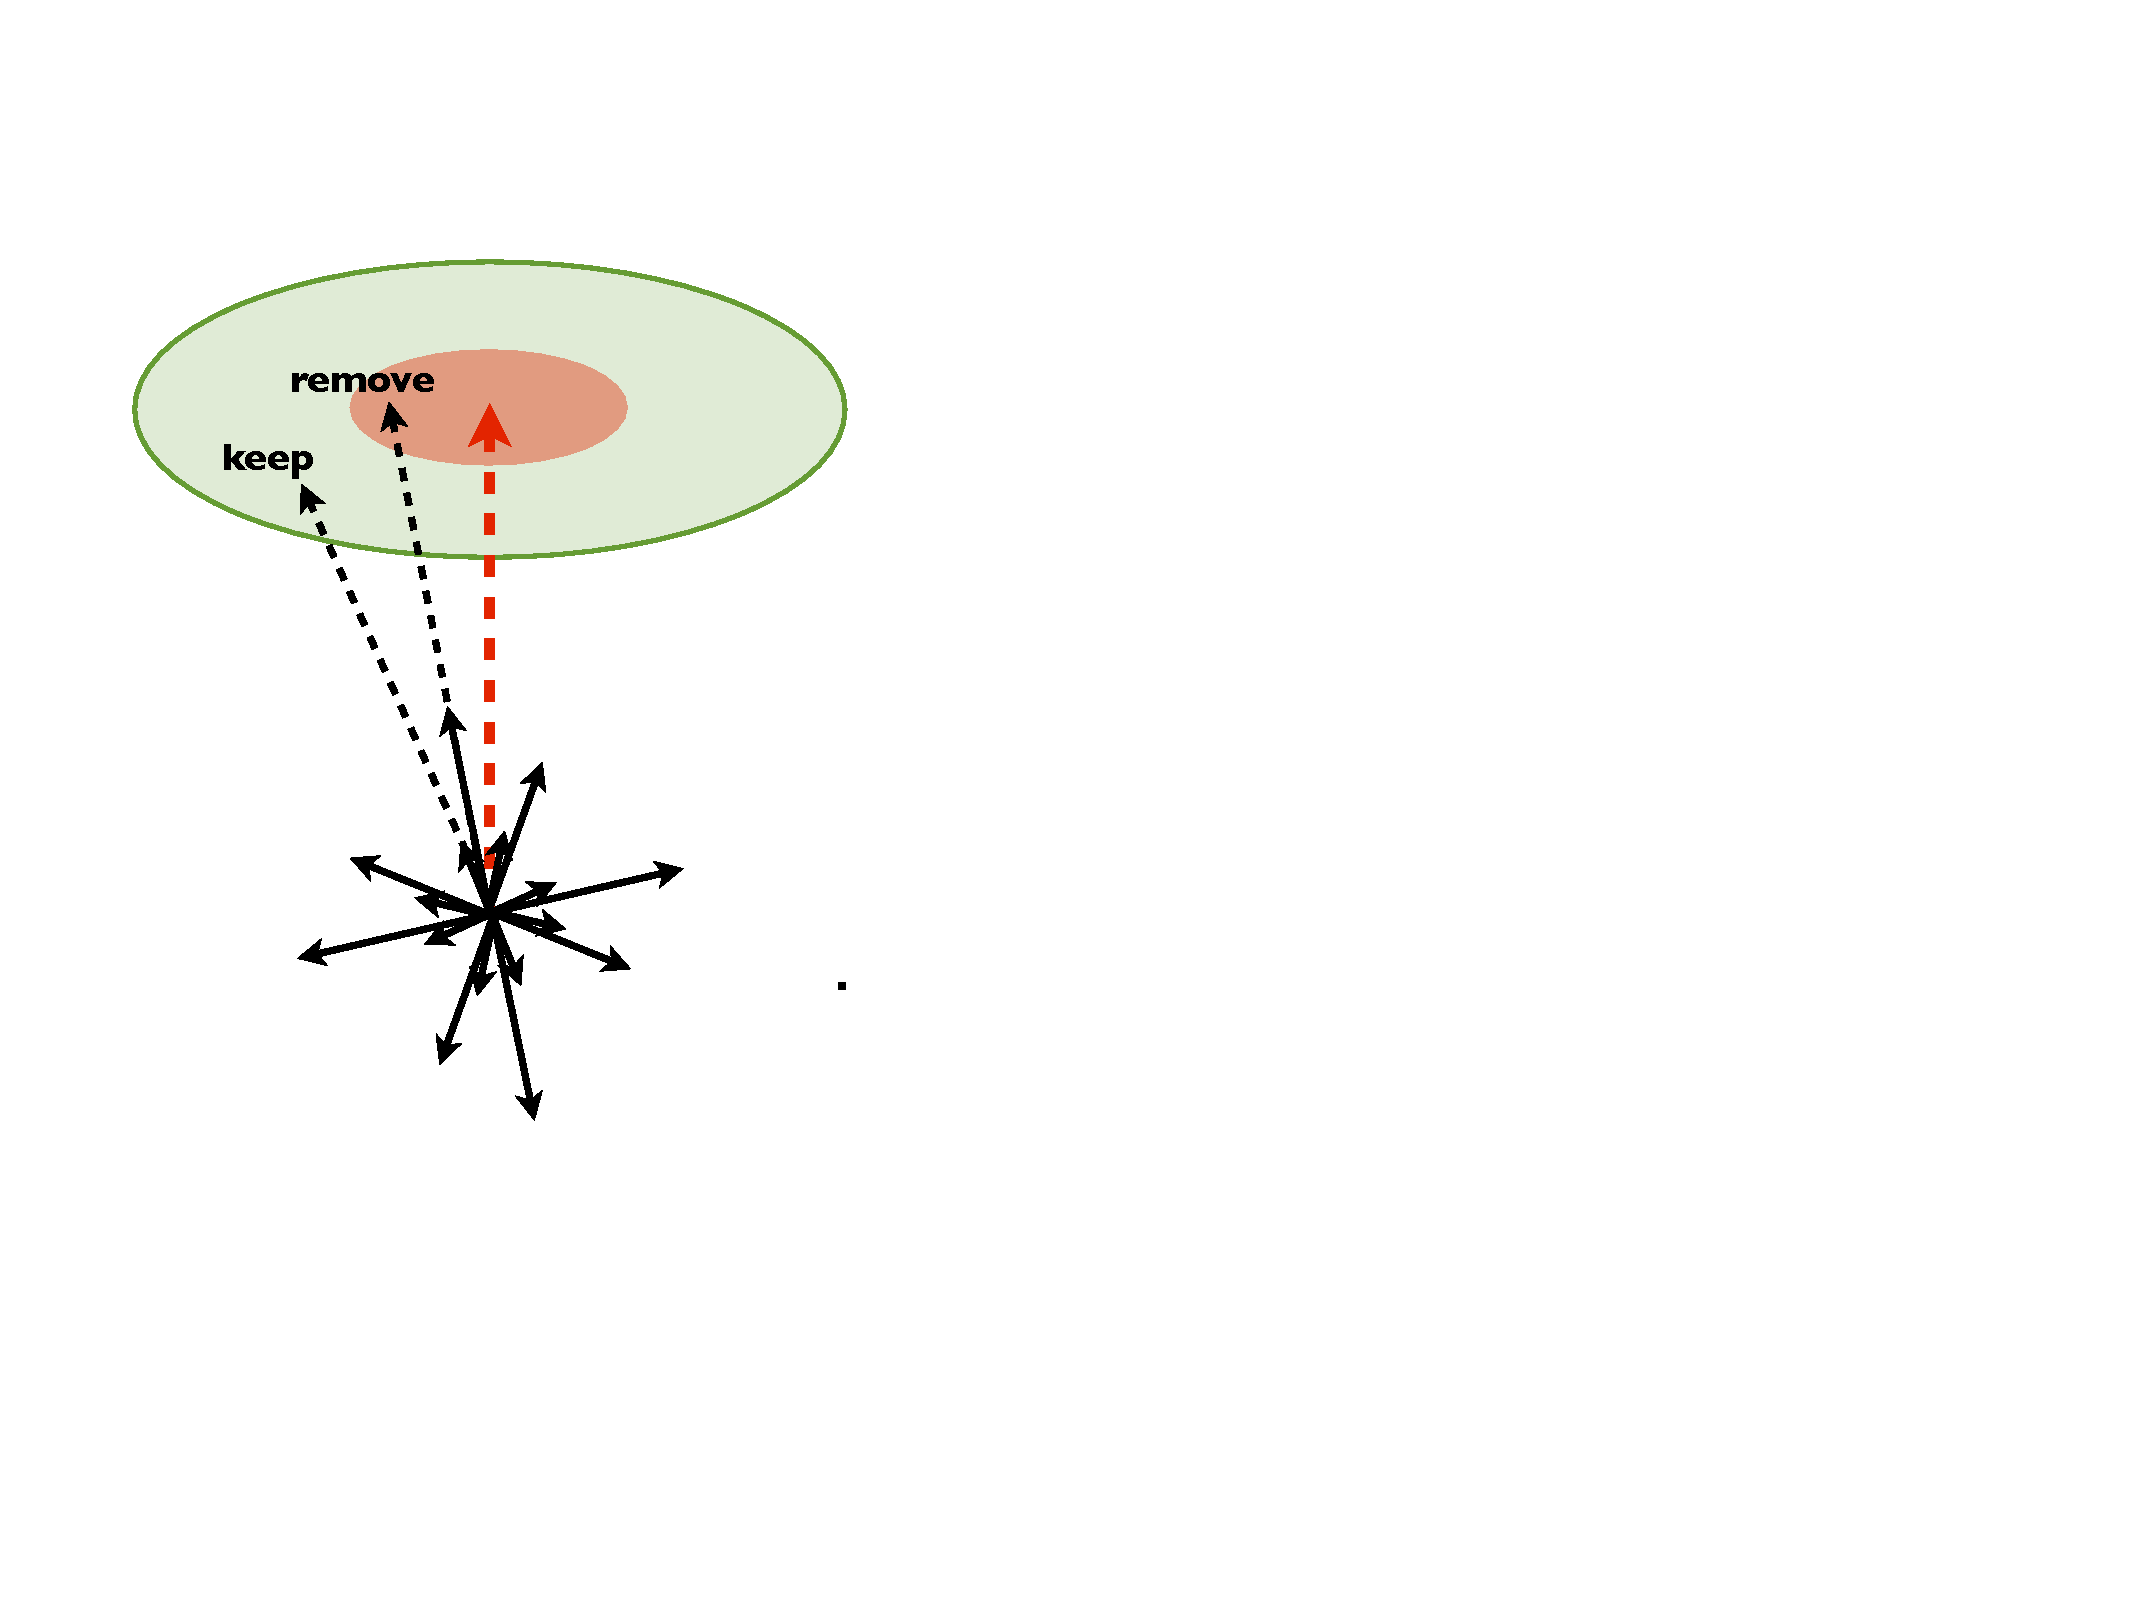
\includegraphics[width=0.4\textwidth]{Figures/RandomCone3.pdf}
\caption{}
\end{center}
\end{figure}

\subsection{Corrections to simulated events}

\section{Jet Selection and b-tag Requirements}

\section{Background Estimation}

\begin{figure} \label{fig-RandomConeIsolation}
\begin{center}
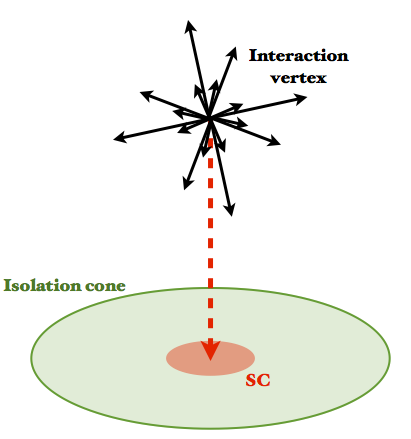
\includegraphics[width=0.45\textwidth]{Figures/RandomCone1.png}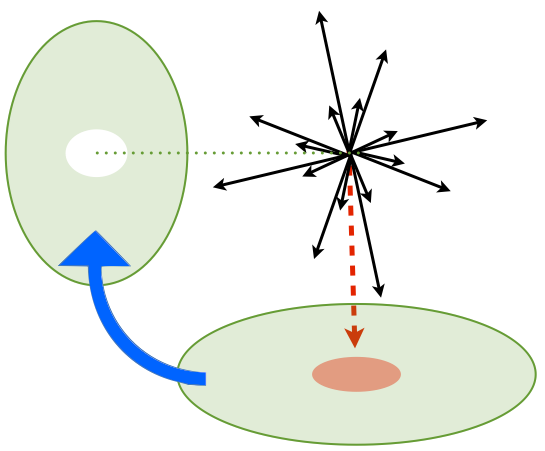
\includegraphics[width=0.55\textwidth]{Figures/RandomCone2.png}
\caption{}
\end{center}
\end{figure}

\begin{sidewaystable} \label{tab-datasets}
\begin{center}
\begin{tabular}{|l|c|c|}
\hline
	\textbf{Dataset} & \textbf{Run Range} & \textbf{Integrated Luminosity ($pb^{-1}$)}\\
\hline
	/DoubleMuParked/Run2012A-22Jan2013-v1/AOD &  & 876 \\
	/DoubleMuParked/Run2012B-22Jan2013-v1/AOD &  & 4412 \\
	/DoubleMuParked/Run2012C-22Jan2013-v1/AOD &  & 7017 \\
	/DoubleMuParked/Run2012D-22Jan2013-v1/AOD &  & 7369 \\
\hline
	Total & & 19.7\\	
\hline
	/DoubleElectron/Run2012A-22Jan2013-v1/AOD &  & 875 \\
	/DoubleElectron/Run2012B-22Jan2013-v1/AOD &  & 4412 \\
	/DoubleElectron/Run2012C-22Jan2013-v1/AOD &  & 7055 \\
	/DoubleElectron/Run2012D-22Jan2013-v1/AOD &  & 7369 \\
\hline
	Total & & 19.7\\	
\hline
	/MuEG/Run2012A-22Jan2013-v1/AOD &  & 876 \\
	/MuEG/Run2012B-22Jan2013-v1/AOD &  & 4411 \\
	/MuEG/Run2012C-22Jan2013-v1/AOD &  & 7055 \\
	/MuEG/Run2012D-22Jan2013-v1/AOD &  & 7360 \\
\hline
	Total & & 19.7\\	
\hline	
\end{tabular}	
\caption{Dataset information for each run in each respective decay channel.}
\end{center}
\end{sidewaystable}

